%%%%%%%%%%%%%%%%%%%%%%%%%%%%%%%%%%%%%%%%%%%%%%%%%%%%%%%%%%%%%%%%%%%%
%%%           Vorlage für eine Ausarbeitung an der DHBW          %%%
%%%                                                              %%%
%%%      Bereiche die bearbeitet werden müssen werden durch      %%%
%%%      einen solchen Kommentarblock eingeleitet und enden      %%%
%%%      mit der nächsten Trennlinie.                            %%%
%%%                                                              %%%
%%%      In dieser Datei müssen folgende Bereiche bearbeitet     %%%
%%%      werden:                                                 %%%
%%%      - Angaben zur Arbeit                                    %%%
%%%      - EIGENE KAPITEL EINFÜGEN                               %%%
%%%                                                              %%%
%%%      Benötigte Seiten und Verzeichnisse können unter         %%%
%%%      "Einführung und Verzeichnisse" ein- bzw. auskommentiert %%%
%%%      werden.                                                 %%%
%%%                                                              %%%
%%%%%%%%%%%%%%%%%%%%%%%%%%%%%%%%%%%%%%%%%%%%%%%%%%%%%%%%%%%%%%%%%%%%

\documentclass[a4paper,12pt]{article}
\usepackage[left=2.5cm,right=2.5cm,top=2.5cm,bottom=2.5cm,includehead]{geometry}      % Einstellungen der Seitenränder
\usepackage[english, ngerman]{babel}                                                  % deutsche Silbentrennung
\usepackage[utf8]{inputenc}                                                           % Umlaute
\usepackage[T1]{fontenc}													                                    % Umlaute auch richtig ausgeben
%\usepackage{newtxtext,newtxmath}                                                      % Font = Times New Roman
\usepackage{hyperref}
\usepackage[nottoc]{tocbibind}
\usepackage{fancyhdr}
\usepackage{setspace}
\usepackage[backend=bibtex, citestyle=authoryear, bibstyle=authoryear]{biblatex}      % Bibliothek für Zitate
\usepackage{csquotes}                                                                 % Zusatzpacket für Zitate
%\usepackage{amsmath}                                                                  % Zurücksetzen der Tabellen- und Abbildungsnummerierung je Sektion
\usepackage[labelfont=bf,aboveskip=1mm]{caption}                                      % Bild- und Tabellenunterschrift (fett)
\usepackage[bottom,multiple,hang,marginal]{footmisc}                                  % Fußnoten [Ausrichtung unten, Trennung durch Seperator bei mehreren Fußnoten]
\usepackage{graphicx}  
\graphicspath{{./images/}}                                                            % Grafiken
\usepackage[dvipsnames]{xcolor}                                                       % Farbige Buchstaben
\usepackage{wrapfig}                                                                  % Bilder in Text integrieren
\usepackage{enumitem}                                                                 % Befehl setlist (Zeilenabstand für itemize Umgebung auf 1 setzen)
\usepackage{listings}                                                                 % Quelltexte
\usepackage{tabularx}                                                                 % Tabellen
\usepackage[addtotoc]{abstract}                                                       % Abstract
\usepackage[nohyperlinks, printonlyused, withpage]{acronym}                           % Abkürzungen

%%%%%%%%%%%%%%%%%%%%%%%%%%%%%%%%%%%%%%%%%%%%%%%%%%%%%%%%%%%%%%%%%%%%
%%%                      Angaben zur Arbeit                      %%%
%%%%%%%%%%%%%%%%%%%%%%%%%%%%%%%%%%%%%%%%%%%%%%%%%%%%%%%%%%%%%%%%%%%%
\def\vFirmenlogoPfad{}                        %% relativer Pfad Bsp.: images/Firmenlogo.png
\def\vDHBWLogoPfad{images/DHBW_logo.jpg}                          %% relativer Pfad Bsp.: images/DHBW_logo.jpg

\def\vTitel{Testtitel}                           %%
\def\vUntertitel{}                      %% 
\def\vArbeitstyp{}                      %% Projektarbeit/Seminararbeit/Bachelorarbeit
\def\vArbeitsbezeichnung{}              %% T1000/T2000/T3000

\def\vAutor{}                           %% Vorname Nachname
\def\vMatrikelnummer{}                  %% 7-stellige Zahl
\def\vKursKuerzel{}                     %% Bsp.: TIT20
\def\vPhasenbezeichnung{}               %% Praxisphase/Theoriephase
\def\vStudienJahr{}                     %% erste/zweite/dritte
\def\vDHBWStandort{}                    %% Bsp.: Ravensburg
\def\vDHBWCampus{}                      %% Bsp.: Friedrichshafen
\def\vFakultaet{}                       %% Technik/Wirtschaft
\def\vStudiengang{}                     %% Informationstechnik/...

\def\vBetrieb{}                         %% 
\def\vBearbeitungsort{}                 %% 
\def\vAbteilung{}                       %% 
\def\vBetreuer{}                        %% Vorname Nachname

\def\vAbgabedatum{\today}               %% DD. MONTH YYYY
\def\vBearbeitungszeitraum{}            %% DD.MM.YYYY - DD.MM.YYYY


%%%%%%%%%%%%%%%%%%%%%%%%% Eigene Kommandos %%%%%%%%%%%%%%%%%%%%%%%%%
% Definition von \gqq{}: Text in Anführungszeichen
\newcommand{\gqq}[1]{\glqq #1\grqq}


%%%%%%%%%%%%%%%%%%%% Zitatbibliothek einbinden %%%%%%%%%%%%%%%%%%%%%
\addbibresource{./literatur/literatur.bib}


%%%%%%%%%%%%%%%%%%%%%%%% PDF-Einstellungen %%%%%%%%%%%%%%%%%%%%%%%%%
\hypersetup{
  bookmarksopen=false,
	bookmarksnumbered=true,
	bookmarksopenlevel=0,
  pdftitle=\vTitel,
  pdfsubject=\vTitel,
  pdfauthor=\vAutor,
  pdfborder={0 0 0},
	pdfstartview=Fit,
  pdfpagelayout=SinglePage
}


%%%%%%%%%%%%%%%%%%%%%%%% Kopf- und Fußzeile %%%%%%%%%%%%%%%%%%%%%%%%
\pagestyle{fancy}
\setlength{\headheight}{15pt}
\fancyhf{}
\fancyhead[R]{\thepage}


%%%%%%%%%%%%%%%%%%%%%%%%%%%%%% Layout %%%%%%%%%%%%%%%%%%%%%%%%%%%%%%
\onehalfspacing
\setlist{noitemsep}

\addto\catpionsngerman{
  \renewcommand{\figurename}{Abb.}
  \renewcommand{\tablename}{Tab.}
}
\numberwithin{table}{section}                               % Tabellennummerierung je Sektion zurücksetzen
\numberwithin{figure}{section}                              % Abbildungsnummerierung je Sektion zurücksetzen
\renewcommand{\thetable}{\arabic{section}.\arabic{table}}   % Tabellennummerierung mit Section
\renewcommand{\thefigure}{\arabic{section}.\arabic{figure}} % Abbildungsnummerierung mit Section
\renewcommand{\thefootnote}{\arabic{footnote}}              % Sektionsbezeichnung von Fußnoten entfernen

\renewcommand{\multfootsep}{, }                             % Mehrere Fußnoten durch ", " trennen


%%%%%%%%%%%%%%%%%%%%%%%%%%%%% Dokument %%%%%%%%%%%%%%%%%%%%%%%%%%%%%

\begin{document}


  %%%%%%%%%%%%%%%%%%% Einführung und Verzeichnisse %%%%%%%%%%%%%%%%%%%
  \pagenumbering{Roman}

  \begin{titlepage}
    \begin{minipage}{6in}
        \vspace*{-2cm}
        \centering
        \hspace{-2cm}
%        \ifx\vFirmenlogoPfad\empty
%        \else
%        \raisebox{-0.5\height}{\includegraphics[height=4cm]{\vFirmenlogoPfad}}
%        \fi
        \hfill
        \ifx\vDHBWLogoPfad\empty
        \else
        \raisebox{-0.5\height}{\includegraphics[height=4cm]{\vDHBWLogoPfad}}
        \fi
    \end{minipage}
    \begin{center}
        \vspace*{0.5cm}
        \Huge\textbf{\vTitel}\\
        \ifx\vUntertitel\empty
        \else
        \Large\textrm{\vUntertitel}\\
        \fi
        \vspace*{2cm}
        \Large\textbf{\vArbeitstyp}
        \ifx\vArbeitsbezeichnung\empty
        \else
        \textbf{\vArbeitsbezeichnung}
        \fi
        \\
        \normalsize
%        über die \vPhasenbezeichnung\ des \vStudienJahr{n}\ Studienjahrs \\
%        \vspace*{1cm}
        an der Fakultät für \vFakultaet\\
        im Studiengang \vStudiengang\\
        \vspace*{0.5cm}
        an der DHBW \vDHBWStandort\\
        \ifx\vDHBWCampus\empty
        \else
        Campus \vDHBWCampus\\
        \fi
        \vspace*{0.5cm}
        von\\
        \ifx\vAutor\empty
        \else
        \vAutor\\
        \fi
        \vspace*{1cm}
        \vAbgabedatum
        \vfill
    \end{center}
    \begin{tabular}{ll}
        Bearbeitungszeitraum:          & \vBearbeitungszeitraum          \\
%        Matrikelnummer, Kurs:          & \vMatrikelnummer, \vKursKuerzel \\
%        Dualer Partner:               & \vBetrieb                       \\
%        Betreuer des Dualen Partners: & \vBetreuer                      \\
    \end{tabular}
\end{titlepage}
\newpage
\setcounter{page}{2}
  % \thispagestyle{empty}
\section*{\Huge{Sperrvermerk}}

\addcontentsline{toc}{section}{Sperrvermerk}
gemäß Ziffer 1.1.13 der Anlage 1 zu §§ 3, 4 und 5  der Studien- und Prüfungsordnung für die Bachelorstudiengänge im Studienbereich Technik der Dualen Hochschule Baden-Würt­tem­berg vom 29.09.2017.\\

\noindent \gqq{Der Inhalt dieser Arbeit darf weder als Ganzes noch in Auszügen Personen außerhalb des Prüfungsprozesses und des Evaluationsverfahrens zugänglich gemacht werden, sofern keine anders lautende Genehmigung vom Dualen Partner vorliegt.}

\vfill
\leavevmode
\newline
\parbox{6cm}{\centering \vBearbeitungsort, \vAbgabedatum\hrule\strut\centering\footnotesize Ort, Datum} 
\hfill
\parbox{6cm}{\hspace{1pt} \vAbteilung\hrule\strut\centering\footnotesize Abteilung, Unterschrift}

\newpage
  \thispagestyle{empty}
\section*{\Huge{Selbstständigkeitserklärung}}

\addcontentsline{toc}{section}{Selbstständigkeitserklärung}
gemäß Ziffer 1.1.13 der Anlage 1 zu §§ 3, 4 und 5  der Studien- und Prüfungsordnung für die Bachelorstudiengänge im Studienbereich Technik der Dualen Hochschule Baden-Würt­tem­berg vom 29.09.2017.

\noindent Ich versichere hiermit, dass ich meine Bachelorarbeit ( bzw.\ Projektarbeit oder Studienarbeit bzw.\ Hausarbeit ) mit dem Thema:
\begin{center}
	\Large\textbf{\vTitel}
\end{center}
selbstständig verfasst und keine anderen als die angegebenen Quellen und Hilfsmittel benutzt habe.
Ich versichere zudem, dass die eingereichte elektronische Fassung mit der gedruckten Fassung übereinstimmt.

\vfill
\leavevmode
\newline
\parbox{6cm}{\centering \vBearbeitungsort, \vAbgabedatum\hrule\strut\centering\footnotesize Ort, Datum} 
\hfill
\parbox{6cm}{\hspace{1pt} \vAbteilung\hrule\strut\centering\footnotesize Abteilung, Unterschrift}

\newpage
  \phantomsection
\newenvironment{keywords}{
	\begin{flushleft}
	\small	
	\textbf{
		\iflanguage{ngerman}{Schlüsselwörter}{\iflanguage{english}{Keywords}{}}
	}
}{\end{flushleft}}

% Deutsche Zusammenfassung
\begin{abstract}
	Das Internet ist aus dem modernen Leben kaum mehr wegzudenken und damit gilt das Selbe für Suchmaschinen wie
	Google, Bing und Co welche das durchforsten des Internets überhaupt erst ermöglichen.
	Um sich die Gunst der Nutzer zu erkämpfen und die stärkste Position in diesem Markt einzunehmen haben sich Suchmaschinen
	stetig weiter entwickelt um den Konkurrenten stets einen Schritt voraus zu sein.

	Ziel dieser Arbeit ist es einen kurzen Überblick über die Geschichte von Suchmaschinen und im Speziellen den Werdegang
	von Google zur meist genutzten Suchmaschine der Welt zu geben, sowie einen eher unbekannten Konkurrenten des
	Internetgiganten zu betrachten und einen kleinen Ausblick auf die potentielle Zukunft von Suchmaschinen zu geben.

	Um dieses Ziel zu erreichen werden in dieser Arbeit die Ergebnisse von einer im Rahmen dieses Projekts durchgeführten
	Konkurrenzanalyse sowie eines Usability-Tests mit Google, Bing und Qwant als betrachteten Zielen dargelegt.
	
\end{abstract}

% Schlüsselwörter Deutsch
\begin{keywords}

\end{keywords}


\selectlanguage{english}
% Englisches Abstract
\begin{abstract}
	To imagine a modern world without the internet is nearly impossible today and therefore the same also goes for search
	engines like Google, Bing and others since they make it even possible to traverse the internet.
	In order to attract the most users and to gain the most influential position in this market search engines have
	constantly evolved in order to always be one step ahead of their competitors.

	The aim of the presented work is to give a brief summary of the history of search engines and in particular how
	Google became the most used search engine in the world, as wall as look at a rather less known competitor of the
	internet giant and give a small glimpse of the potential future of search engines.

	In order to do so the presented work will showcase the results of a competitor analysis as well as a usability test
	with Google, Bing and Qwant as their targets, that were conducted as part of this project.
\end{abstract}

% Schlüsselwörter Englisch
\begin{keywords}

\end{keywords}


\selectlanguage{ngerman}
\newpage
  \tableofcontents
\newpage
  \section*{Abkürzungsverzeichnis}
\addcontentsline{toc}{section}{Abkürzungsverzeichnis}
\begin{acronym}
  \acro{DHBW}[DHBW]{Duale Hochschule Ba\-den-\-Würt\-tem\-berg}
  \acroplural{DHBW}[DHBW]{Dualen Hochschule Ba\-den-\-Würt\-tem\-berg}

  \acro{WCAG}[WCAG]{Web Content Accessibility Guidelines}
\end{acronym}
\newpage
  \listoffigures
\newpage
  \listoftables
\newpage
  % \section*{Vorwort}
\addcontentsline{toc}{section}{Vorwort}
\newpage


  %%%%%%%%%%%%%%%%%%%%%%%%%%%%% Kapitel %%%%%%%%%%%%%%%%%%%%%%%%%%%%%%
  \pagestyle{fancy}
  \fancyhead[L]{\nouppercase{\rightmark}}    % Abschnittsname im Header
  \pagenumbering{arabic}

  %%%%%%%%%%%%%%%%%%%%%%%%%%%%%%%%%%%%%%%%%%%%%%%%%%%%%%%%%%%%%%%%%%%%
  %%%%                   EIGENE KAPITEL EINFÜGEN                  %%%%
  %%%%%%%%%%%%%%%%%%%%%%%%%%%%%%%%%%%%%%%%%%%%%%%%%%%%%%%%%%%%%%%%%%%%
  \section{Einleitung}\label{sec:einleitung}
Wie kann Google den Markt der Suchmaschinen mit über 90 Prozent Marktanteil so stark dominieren und welche Konkurrenz gibt es?
Wäre baldiger Wechsel an der Spitze des Marktes denkbar?
In der folgenden Arbeit soll der Markt der Suchmaschinen und einzeln ausgewählte Vertreter analysiert werden.
Um die Situation auf dem Markt zu verstehen und die wichtigsten Punkte kennenzulernen, in denen sich eine Suchmaschine beweisen muss,
wird im Folgenden zuerst eine Konkurrenzanalyse durchgeführt, bei der zum einen der \("\)big-player\("\) Google,
aber auch der Konkurrent Bing und eine Start-up-Suchmaschine namens Qwant betrachtet werden.
Um die Konkurrenzsituation genau zu erläutern werden hier verschiedene Aspekte der Suchmaschinen untersucht, analysiert und dann einander gegenüber gestellt.
Fortlaufend wird im zweiten Kapitel herausgearbeitet wie Google schon früh aus der Menge der Suchmaschinen herausstach und den Markt bis heute dominiert.
Hierbei wird Googles Strategie zu unterschiedlichen Zeitpunkten bewertet und untersucht, wie sie auf die heutige Topposition der Suchmaschine einwirkten.
Vom \("\)big-player\("\) zu einer bisher ziemlich kleinen, unbekannten Suchmaschine,
wird dann das französische Start-up Qwant betrachtet, wessen Suchmaschine sich trotz eines bisher kleinen Marktanteils großer Beliebtheit erfreut.
Dabei werden die Gründe für den Erfolg von Qwant, seine Chancen und Vorteile gegenüber der bereits genannten Konkurrenz herausgearbeitet.
Ein wichtiger Aspekt für Suchmaschinen ist ihre Finanzierung, da diese oft gar nicht so offensichtlich ist.
Folgend werden im vierten Kapitel die verschiedenen Finanzierungskonzepte und ihre Rolle in der Aufstellung am Markt untersucht.
Um die praktische Erfahrung mit den Suchmaschinen Google, Bing und Qwant herauszuarbeiten werden im Anschluss die Ergebnisse von Usability-Tests mit den drei Anbietern präsentiert.
Diese sollen die Anwendung der Suchmaschinen im Alltag analysieren und so weitere Aspekte, Vor- und Nachteile einzelner Anbieter aufzeigen.
Zuletzt wird betrachtet, wie Suchmaschinen, vor allem Google, uns als Nutzer beeinflusst oder schon beeinflusst hat.
Auch soll hier ein Blick in die Zukunft geworfen werden und betrachtet werden, wie Google und Co uns weiter beeinflussen könnten und welche Rolle sie in der Zukunft spielen könnten.
  \section{Wie uns Google beeinflusst}\label{sec:wie-uns-google-beeinflusst}

\subsection{Der Einfluss von Google}\label{subsec:der-einfluss-von-google}
Mit einem Marktanteil von über 90 Prozent in Deutschland, im mobilen Sektor sogar über 96 Prozent, erfreut sich die Google Suchmaschine in den letzten Jahren immer größerer Beliebtheit.
Während das Rennen der Suchmaschinen vor etwa 20 Jahren noch ein \("\)bunte Mischung\("\) war, hat Google heute nahezu ein Monopol in diesem Bereich geschaffen.
Auch weltweit ist Google, wenn auch nicht so eindeutig wie das in Deutschland der Fall ist, mit Abstand auf Platz eins der beliebtesten Suchmaschinen.
Jeder von uns \("\)googelt\("\)\cite{DUD22}, wie es die Suchmaschine schon in den deutschen Duden geschafft hat, im Schnitt dreimal am Tag.\cite{DOL22}\\
Wenn man diese Zahlen hört, dürfte schon klar sein, dass Google unser Verhalten als Nutzer im Web maßgeblich beeinflusst hat.
Wie genau Google uns beeinflusst hat oder vielleicht noch beeinflussen wird, wird im Folgenden analysiert.

\subsection{Veränderung des Benutzerverhaltens mehrerer Generationen}\label{subsec:veränderung-des-benutzerverhaltens-mehrerer-generationen}
Modernisierung des Webs - das Google-Ranking bestimmt, ob und auf welchem Platz eine Webseite dem Nutzer bei einer Suchanfrage vorgeschlagen wird.
Um in diesem Ranking möglichst gut platziert zu werden, sollte man bestimmte Voraussetzungen erfüllen, so sei es beispielsweise wichtig die Webseite gut an die Ansicht auf Mobilen Geräten anzupassen.\cite{BUI22}
Wie eine Statistik von statcounter zeigt, übertraf die Internetnutzung auf mobilen Geräten 2016 erstmals die Nutzung von einem Desktop aus mit einem ständigen Wachstum der mobilen Nutzung seit 2009.\cite{STA16}
Nicht zuletzt dürfte dazu wohl auch die immer besser werdende Benutzerfreundlichkeit von Webseiten auf mobilen Geräten beigetragen haben.
Und weil Seiten mit einer guten Anpassung auf mobile Geräte von Google höher gerankt werden, ist es wohl kein Wunder, dass wir unsere mobilen Geräte auch für das surfen im Netz immer mehr benutzen können.
Auch in Zukunft, wenn der Trend weiter in Richtung mobile Geräte, wie eventuell auch SmartWatches oder Sprachsteuerung geht,
wird Google wohl signifikant mitbestimmen, inwieweit das World Wide Web zugänglich für neue Technologien wird.\\

Informationsbeschaffung - Informationsquellen, die Quellen, aus denen wir unser Individualwissen nehmen,
veränderten und vermischten sich in der Geschichte immer wieder aufs Neue.
Von reiner mündlicher Überlieferung über Buchdruck und Radio bis zum Fernsehen.
Doch wohl kaum gab es zuvor eine Quelle mit der man so schnell Informationen in vergleichbaren Mengen und aus vergleichbar vielen Quellen beschaffen konnte wie mit dem Internet.
Einem Bericht der \("\)mednic\("\) zufolge gaben 82 Prozent der Befragten 2020 an sich über Covid-19 im Internet zu informieren.\cite{RKW20}
Ob über Nachrichtenseiten, Social Media oder Podcasts und egal über welches Thema,
Google und Co liefern uns Informationen und vor allem in jüngeren Generationen werden Suchmaschinen eine immer beliebtere Informationsquelle.\\

Konnektivität der Google Dienste - ob die Google Suchmaschine, Gmail, YouTube, Maps oder den Google Play Store,
die meisten von uns nutzen nicht nur eines der zahlreichen Google Produkte und Dienste.
In der Gmail-App kann man ganz einfach mithilfe von Google Drive auch größere Dateien anhängen und in der Google Suchmaschine kann man ganz einfach seinen YouTube und Gmail Account einbinden, alles mit Hilfe des Google Kontos.
Und das sind nur ein paar Beispiele, wie man verschiedenste Google Dienste vergleichsweise einfach miteinander verbinden kann.
\begin{figure}[ht]
    \centering
    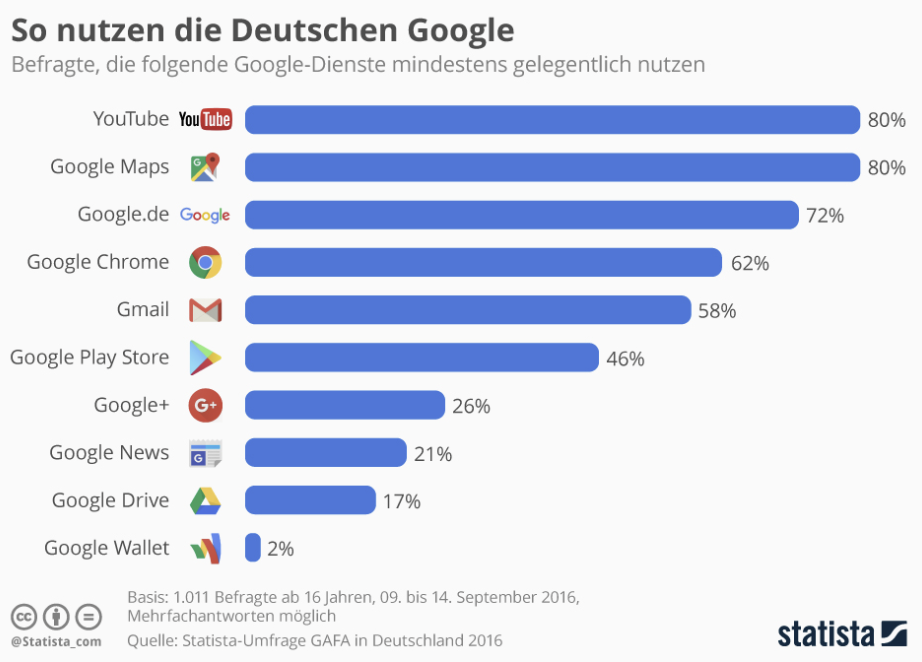
\includegraphics[width=100mm]{images/statistic_googleServices}
    \caption{Statistik Nutzung der Google Dienste in Deutschland}
    \label{fig:statisticGoogleServices}
\end{figure}  %https://de.statista.com/infografik/6020/nutzung-von-google-diensten-in-deutschland/
Wie in der Statistik zu sehen ist, nutzen bereits heute 80 Prozent der Menschen in Deutschland Google Maps und YouTube, dicht gefolgt von der Google Suchmaschine mit 72 Prozent.
Auch die restlichen Google Services sind in Deutschland gut vertreten und das wohl nicht zuletzt auch,
weil Google es uns in den letzten Jahren immer einfacher gemacht hat die verschiedenen Dienste miteinander zu verbinden.
Erst 2019 wurde Google+, was immerhin 26 Prozent der Deutschen nutzten, eingestellt.
Bei dem Google Dienst, der gerade einmal knapp 8 Jahre am Markt war, handelte es sich um ein soziales Netzwerk,
das \("\)mehrere Google-Werkzeuge [\ldots] in einem einzigen sozialen Netzwerk von Google\("\)\cite{JEC21} vereinen sollte.\cite{JEC21}
Und, auch wenn dieses Projekt gescheitert ist, sieht man daran, wie Google immer wieder versucht seine Dienste noch besser miteinander zu vernetzen.
Schon heute haben sich die Google features wie wohl kaum eines anderen Anbieter in unseren Alltag integriert,
und so wird Google wohl auch in Zukunft, wenn es vielleicht noch weitere Google Dienste geben wird, durch gute Konnektivität und eine dadurch verbesserte User Experience überzeugen.\\

UX und Einfachheit - Eine schlichte, meist weiße Webseite mit einer Suchbar in der Mitte und einem kleinen Bild darüber,
in den Grundzügen sieht die Landingpage der Google Suchmaschine schon seit es sie gibt so aus.
Mit kleinen der Zeit angepassten Modernisierungen selbstverständlich.
Die Nutzung der Google Suchmaschine könnte wohl kaum einfacher und selbsterklärender sein.
Usability beschreibt die Nutzbarkeit oder auch Gebrauchstauglichkeit eines Produktes und ist ein wesentlicher Bestandteil der UX (=User Experience),
die wiederum beschreibt wie gut die Erfahrung ist, die ein User mit dem Produkt im Durchschnitt macht, also wie einfach und komfortable ein Produkt für der User oder Anwender nutzbar ist.\cite{Maulhardt4}
Durch die einfache und selbsterklärende Nutzung weißt Google eine ziemlich hohe Usability vor und nicht nur das,
die Usability ist auch ein wesentlicher Bestandteil des Rankings von Google, so gibt uns Google bevorzugt Ergebnisse aus, bei denen die Usability auch vergleichsmäßig hoch ist,
was ein weiterer Grund ist warum viele die Suchergebnisse von Google sehr schätzen und wohl auch in Zukunft noch schätzen werden.\cite{LIC15}\\

Accessibility der Information - Das Ziel, das die Google Suchmaschine von Anfang an verfolgt hat,
ist es Informationen für Menschen erreichbar zu machen und die Benutzer sind es gewohnt und erwarten auch schnell und einfach an die Information zu kommen.
\begin{figure}[h]
    \centering
    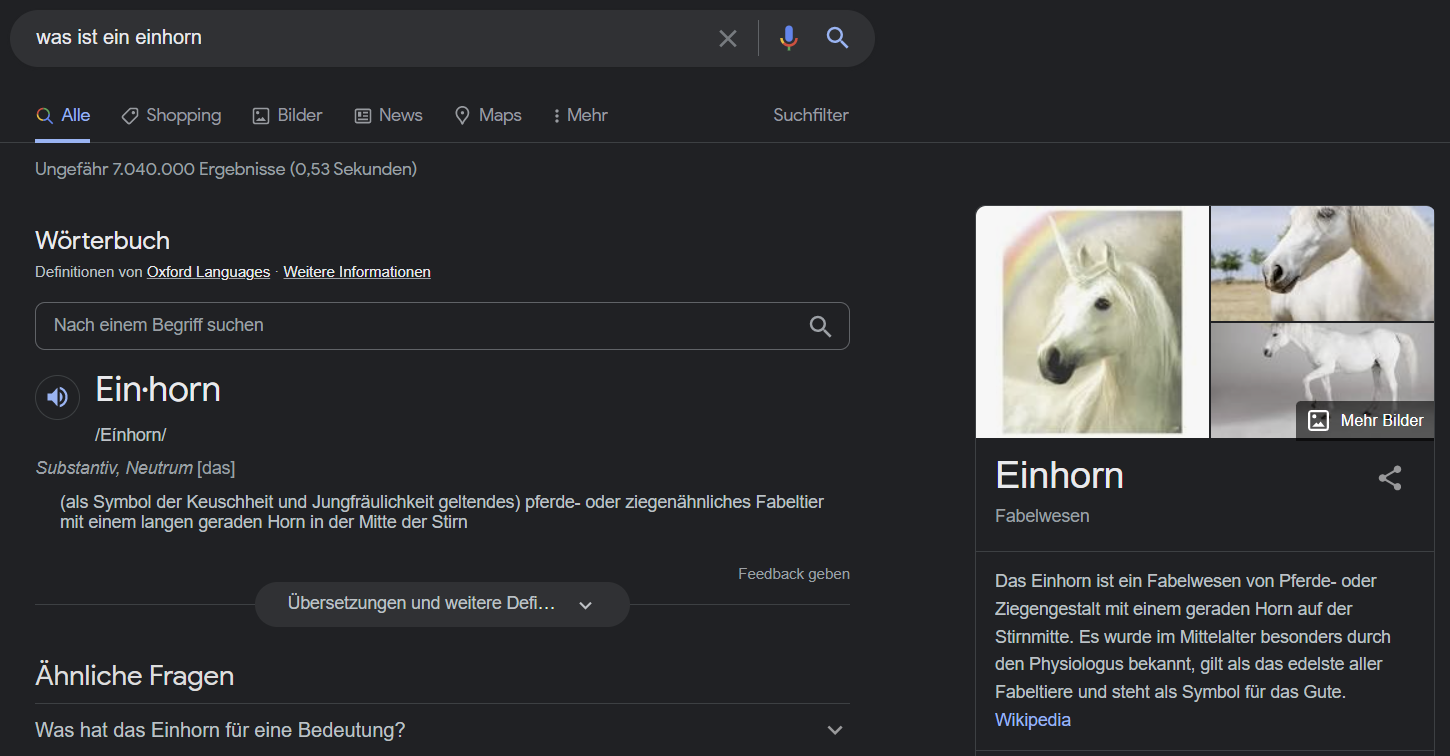
\includegraphics[width=80mm]{images/screenshot_googleQue}
    \caption{Suchergebnis Google}
    \label{fig:screenshotGoogleQue}
\end{figure}
\begin{figure}[h]
    \centering
    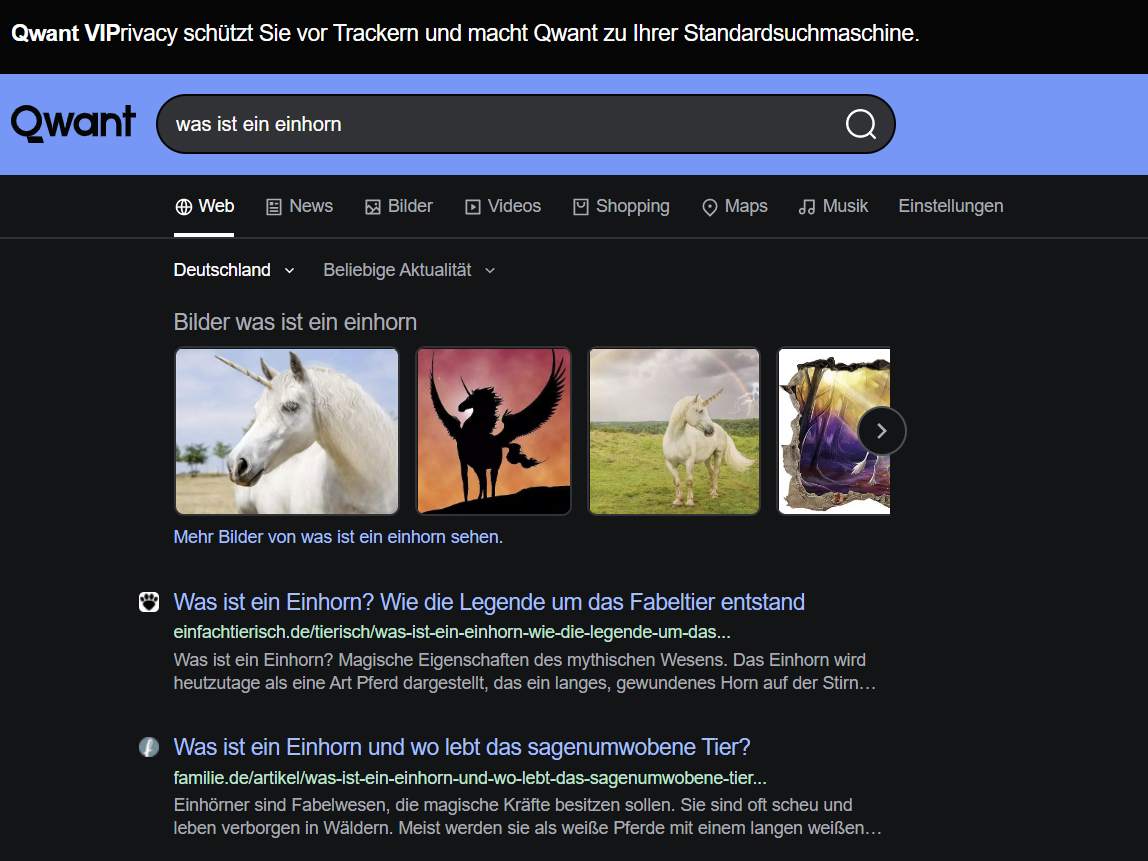
\includegraphics[width=80mm]{images/screenshot_qwantQue}
    \caption{Suchergebnis Qwant}
    \label{fig:screenshotQwantQue}
\end{figure}
Wie man in den angeführten Screenshots sieht, gibt Google direkt die Informationen aus, wo man zum Beispiel bei Qwant zuerst eine Webseite aufrufen muss.
Heute erwarten wir möglichst schnell an die Information zu kommen, worauf sich Google schon angepasst hat.
  \section{Finanzierungskonzepte von Browsern}\label{sec:finanzierungskonzepte-von-browsern}

\subsection{Rückblick}\label{subsec:rueckblick}
Schon im Jahr 2005, als Google gerade einmal 7 Jahre alt war,
kommentierte Prof. Dr. Jens Wolling die Finanzierung von Suchmaschinen mit
\("\)Eine Finanzierung [\ldots] allein aus Bannerwerbung ist unrealistisch\("\)\cite{WOL05},
als weitere Finanzierungsquelle der privatwirtschaftlichen Großkonzerne führt er deshalb Verkauf von Technologie oder
Suchergebnissen an.\cite{WOL05}\\

Den Trend zur damaligen Zeit analysiert er folgendermaßen: Es gäbe zwei mögliche Richtungen, in die Finanzierung der Suchportale entwickeln könnte und es zum Teil auch schon tut.
Die erste Möglichkeit seien Aufnahmegebühren, in diesem Fall müssten Anbieter bezahlen, um überhaupt erst von der Suchmaschine gefunden zu werden.
Die zweite Möglichkeit hingegen seien Platzierungsgebühren, wobei man für eine gute Platzierung bezahlen müsse.
Beide Varianten sieht Wolling durchaus kritisch.\cite{WOL05}\\

Doch wie werden die großen Suchmaschinen und Mediengiganten heute finanziert?
Und wie finanzieren sich Start-ups und kleinere Unternehmen auf dem Markt?
Im Folgenden werden wichtigsten Finanzierungsmöglichkeiten analysiert.

\subsection{Finanzierung durch Werbung}\label{subsec:finanzierung-durch-werbung}
Werbung ist, wie wohl den meisten klar ist eines der größten Standbeine von Google und Co,
so hat Google, wie in der Statistik zu sehen, im Jahr 2021 einen Rekordumsatz von über 200 Milliarden US Dollar durch Werbung umgesetzt, mit einer stetig starken Steigerung der Umsatzes seit 2001.
Auch bei Bing und anderen großen Suchmaschinen sieht die Steigerung ähnlich aus, wenn auch in kleinerem Ausmaß.
\begin{figure}[h]
    \centering
    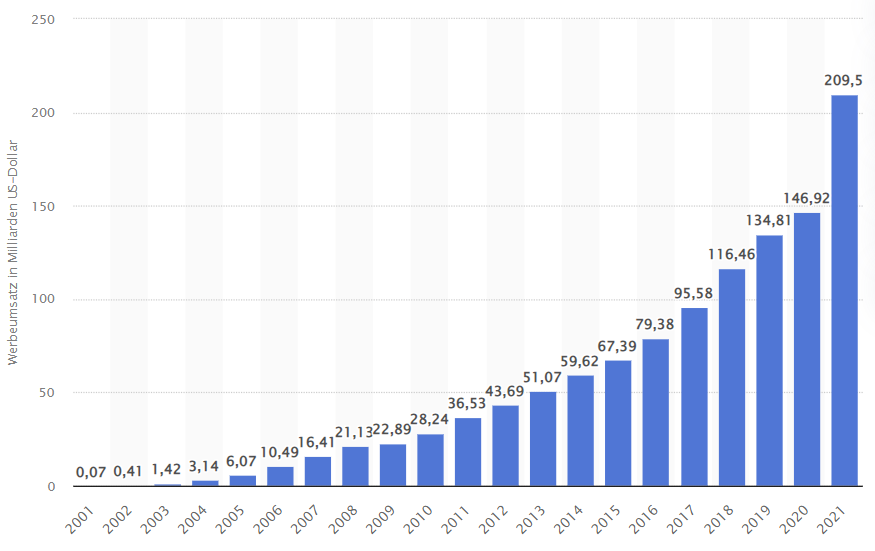
\includegraphics[width=120mm]{images/statistic_google_ads}
    \caption{Statistik Werbeumsätze Google in Milliarden}
    \label{fig:statisticAdsGoogle}
\end{figure}
Besonders in den letzten Jahren wurde auch personalisierte Werbung immer populärer.
Der Journalist und Author Dr. Björn Brückerhoff berichtet in einem Artikel 2020, wie Google Daten aus nahezu allen Anwendungen, sowie der Suchmaschine selbst und Betriebssystemen, wie in etwa Android, nutzt um Persönlichkeitsprofile seiner Nutzer zu erstellen.
Google kann laut Brückerhoff mit Hilfe dieser gigantischen Mengen an Daten auf \("\)Wünsche und Bedürfnisse,
die sexuelle Orientierung, die physische und psychische Gesundheit, die politischen Meinungen, die fnanziellen Möglichkeiten, die religiösen Überzeugungen oder die räumliche Flexibilität\("\)\cite{BRK20} schließen.
Mit Hilfe dieser Persönlichkeitsdaten platziert Google dann die mit Hilfe von Algorithmen ermittelte,
am besten auf uns zugeschnittene Werbung.\cite{BRK20}\\

Das Suchmaschinen-StartUp \("\)Qwant\("\) aus Frankreich gibt hingegen auf der Homepage der eigenen Suchmaschine nicht nur an,
keinerlei persönliche Daten zu verkaufen oder zu Werbezwecken zu nutzen, sondern auch diese persönlichen Daten nicht einmal zu erheben.
Die Suchmaschine finanziert sich laut Webseite \("\)kontextbasierte Werbung[, die] für alle gleich [ist]\("\)\cite{QWA22},
jeder sieht also, unabhängig vorherigen Suchen, die gleiche Werbung.

Bei Ergebnissen zu Suchanfragen kann bei den meisten Suchmaschinen, so auch bei Google,
Bing und Qwant zwischen \("\)Anzeigen\("\) und \("\)organischen Treffern\("\) unterschieden werden.
Anzeigen, auch unter dem Begriff \("\)Paid Listings\("\) bekannt, bezeichnen bezahlte Suchtreffer,
die von Suchmaschinen in die Suchergebnisse \("\)gemischt\("\) werden.
Solche Anzeigen müssen nach EU-Recht als solche gekennzeichnet werden.\\
Organische Treffer sind hingegen Treffer, die durch Algorithmen der Suchmaschine als am besten passend auf die aktuelle Suche bewertet werden.
In der folgenden Statistik wird die Anzahl der als \("\)Anzeige\("\) gekennzeichneten Treffern unter den ersten zehn Treffern auf ausgewählten Suchanfragen gezeigt.\cite{LEW18}\\
\begin{figure}[h]
    \centering
    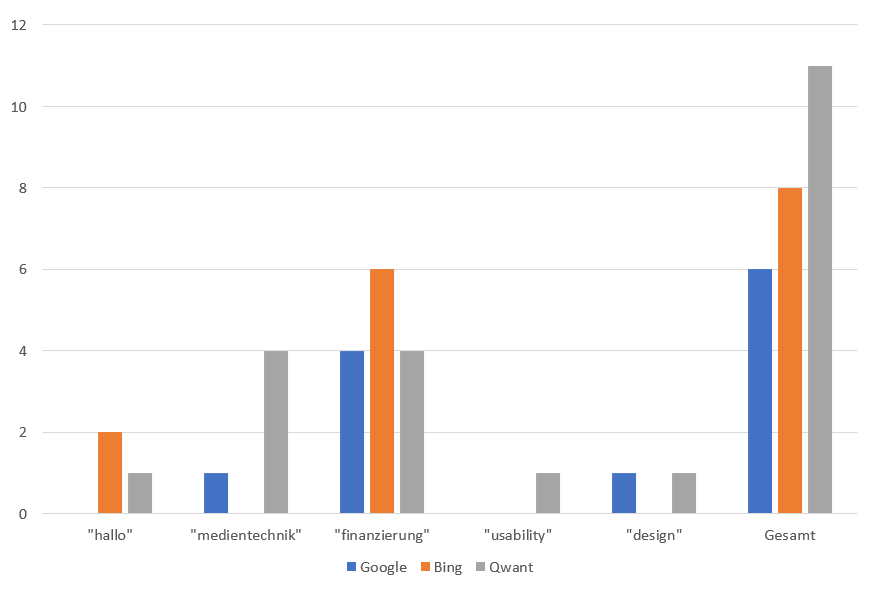
\includegraphics[width=120mm]{images/statistic_adverts}
    \caption{Statistik Anzeigen unter den ersten zehn Treffern bei ausgewählten Suchanfragen}
    \label{fig:statisticAdverts}
\end{figure}
Auffallend ist, dass Qwant insgesamt die meisten Anzeigen platziert hat, was allerdings daraus resultieren könnte,
dass es angibt keine Cookies wie Google und Bing zu verwenden, weshalb eine signifikante Einnahmequelle der Konkurrenz bei Qwant ausfällt.
Schaut man sich die Platzierungen der Anzeigen an, so fällt auf, dass Qwant diese oft,
im Gegensatz zu Bing und Google am Ende der aufgezeigten Suchergebnisse zeigt.
Auch fällt auf, dass der Anbieter mit den meisten Anzeigen bei fast jeder Anzeige sehr unterschiedlich ausfällt,
weshalb das Ergebnis auch stark von den gewählten Suchbegriffen abhängen könnte.\\
  \section{Wie uns Google beeinflusst}\label{sec:wie-uns-google-beeinflusst}

\subsection{Der Einfluss von Google}\label{subsec:der-einfluss-von-google}
Mit einem Marktanteil von über 90 Prozent in Deutschland, im mobilen Sektor sogar über 96 Prozent, erfreut sich die Google Suchmaschine in den letzten Jahren immer größerer Beliebtheit.
Während das Rennen der Suchmaschinen vor etwa 20 Jahren noch ein \("\)bunte Mischung\("\) war, hat Google heute nahezu ein Monopol in diesem Bereich geschaffen.
Auch weltweit ist Google, wenn auch nicht so eindeutig wie das in Deutschland der Fall ist, mit Abstand auf Platz eins der beliebtesten Suchmaschinen.
Jeder von uns \("\)googelt\("\)\cite{DUD22}, wie es die Suchmaschine schon in den deutschen Duden geschafft hat, im Schnitt dreimal am Tag.\cite{DOL22}\\
Wenn man diese Zahlen hört, dürfte schon klar sein, dass Google unser Verhalten als Nutzer im Web maßgeblich beeinflusst hat.
Wie genau Google uns beeinflusst hat oder vielleicht noch beeinflussen wird, wird im Folgenden analysiert.

\subsection{Veränderung des Benutzerverhaltens mehrerer Generationen}\label{subsec:veränderung-des-benutzerverhaltens-mehrerer-generationen}
Modernisierung des Webs - das Google-Ranking bestimmt, ob und auf welchem Platz eine Webseite dem Nutzer bei einer Suchanfrage vorgeschlagen wird.
Um in diesem Ranking möglichst gut platziert zu werden, sollte man bestimmte Voraussetzungen erfüllen, so sei es beispielsweise wichtig die Webseite gut an die Ansicht auf Mobilen Geräten anzupassen.\cite{BUI22}
Wie eine Statistik von statcounter zeigt, übertraf die Internetnutzung auf mobilen Geräten 2016 erstmals die Nutzung von einem Desktop aus mit einem ständigen Wachstum der mobilen Nutzung seit 2009.\cite{STA16}
Nicht zuletzt dürfte dazu wohl auch die immer besser werdende Benutzerfreundlichkeit von Webseiten auf mobilen Geräten beigetragen haben.
Und weil Seiten mit einer guten Anpassung auf mobile Geräte von Google höher gerankt werden, ist es wohl kein Wunder, dass wir unsere mobilen Geräte auch für das surfen im Netz immer mehr benutzen können.
Auch in Zukunft, wenn der Trend weiter in Richtung mobile Geräte, wie eventuell auch SmartWatches oder Sprachsteuerung geht,
wird Google wohl signifikant mitbestimmen, inwieweit das World Wide Web zugänglich für neue Technologien wird.\\

Informationsbeschaffung - Informationsquellen, die Quellen, aus denen wir unser Individualwissen nehmen,
veränderten und vermischten sich in der Geschichte immer wieder aufs Neue.
Von reiner mündlicher Überlieferung über Buchdruck und Radio bis zum Fernsehen.
Doch wohl kaum gab es zuvor eine Quelle mit der man so schnell Informationen in vergleichbaren Mengen und aus vergleichbar vielen Quellen beschaffen konnte wie mit dem Internet.
Einem Bericht der \("\)mednic\("\) zufolge gaben 82 Prozent der Befragten 2020 an sich über Covid-19 im Internet zu informieren.\cite{RKW20}
Ob über Nachrichtenseiten, Social Media oder Podcasts und egal über welches Thema,
Google und Co liefern uns Informationen und vor allem in jüngeren Generationen werden Suchmaschinen eine immer beliebtere Informationsquelle.\\

Konnektivität der Google Dienste - ob die Google Suchmaschine, Gmail, YouTube, Maps oder den Google Play Store,
die meisten von uns nutzen nicht nur eines der zahlreichen Google Produkte und Dienste.
In der Gmail-App kann man ganz einfach mithilfe von Google Drive auch größere Dateien anhängen und in der Google Suchmaschine kann man ganz einfach seinen YouTube und Gmail Account einbinden, alles mit Hilfe des Google Kontos.
Und das sind nur ein paar Beispiele, wie man verschiedenste Google Dienste vergleichsweise einfach miteinander verbinden kann.
\begin{figure}[ht]
    \centering
    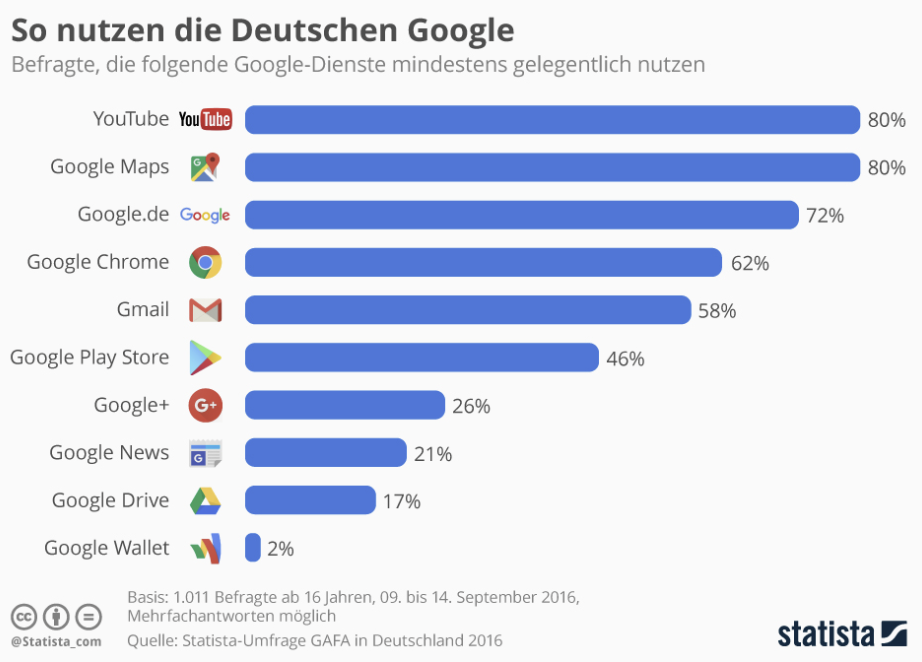
\includegraphics[width=100mm]{images/statistic_googleServices}
    \caption{Statistik Nutzung der Google Dienste in Deutschland}
    \label{fig:statisticGoogleServices}
\end{figure}  %https://de.statista.com/infografik/6020/nutzung-von-google-diensten-in-deutschland/
Wie in der Statistik zu sehen ist, nutzen bereits heute 80 Prozent der Menschen in Deutschland Google Maps und YouTube, dicht gefolgt von der Google Suchmaschine mit 72 Prozent.
Auch die restlichen Google Services sind in Deutschland gut vertreten und das wohl nicht zuletzt auch,
weil Google es uns in den letzten Jahren immer einfacher gemacht hat die verschiedenen Dienste miteinander zu verbinden.
Erst 2019 wurde Google+, was immerhin 26 Prozent der Deutschen nutzten, eingestellt.
Bei dem Google Dienst, der gerade einmal knapp 8 Jahre am Markt war, handelte es sich um ein soziales Netzwerk,
das \("\)mehrere Google-Werkzeuge [\ldots] in einem einzigen sozialen Netzwerk von Google\("\)\cite{JEC21} vereinen sollte.\cite{JEC21}
Und, auch wenn dieses Projekt gescheitert ist, sieht man daran, wie Google immer wieder versucht seine Dienste noch besser miteinander zu vernetzen.
Schon heute haben sich die Google features wie wohl kaum eines anderen Anbieter in unseren Alltag integriert,
und so wird Google wohl auch in Zukunft, wenn es vielleicht noch weitere Google Dienste geben wird, durch gute Konnektivität und eine dadurch verbesserte User Experience überzeugen.\\

UX und Einfachheit - Eine schlichte, meist weiße Webseite mit einer Suchbar in der Mitte und einem kleinen Bild darüber,
in den Grundzügen sieht die Landingpage der Google Suchmaschine schon seit es sie gibt so aus.
Mit kleinen der Zeit angepassten Modernisierungen selbstverständlich.
Die Nutzung der Google Suchmaschine könnte wohl kaum einfacher und selbsterklärender sein.
Usability beschreibt die Nutzbarkeit oder auch Gebrauchstauglichkeit eines Produktes und ist ein wesentlicher Bestandteil der UX (=User Experience),
die wiederum beschreibt wie gut die Erfahrung ist, die ein User mit dem Produkt im Durchschnitt macht, also wie einfach und komfortable ein Produkt für der User oder Anwender nutzbar ist.\cite{Maulhardt4}
Durch die einfache und selbsterklärende Nutzung weißt Google eine ziemlich hohe Usability vor und nicht nur das,
die Usability ist auch ein wesentlicher Bestandteil des Rankings von Google, so gibt uns Google bevorzugt Ergebnisse aus, bei denen die Usability auch vergleichsmäßig hoch ist,
was ein weiterer Grund ist warum viele die Suchergebnisse von Google sehr schätzen und wohl auch in Zukunft noch schätzen werden.\cite{LIC15}\\

Accessibility der Information - Das Ziel, das die Google Suchmaschine von Anfang an verfolgt hat,
ist es Informationen für Menschen erreichbar zu machen und die Benutzer sind es gewohnt und erwarten auch schnell und einfach an die Information zu kommen.
\begin{figure}[h]
    \centering
    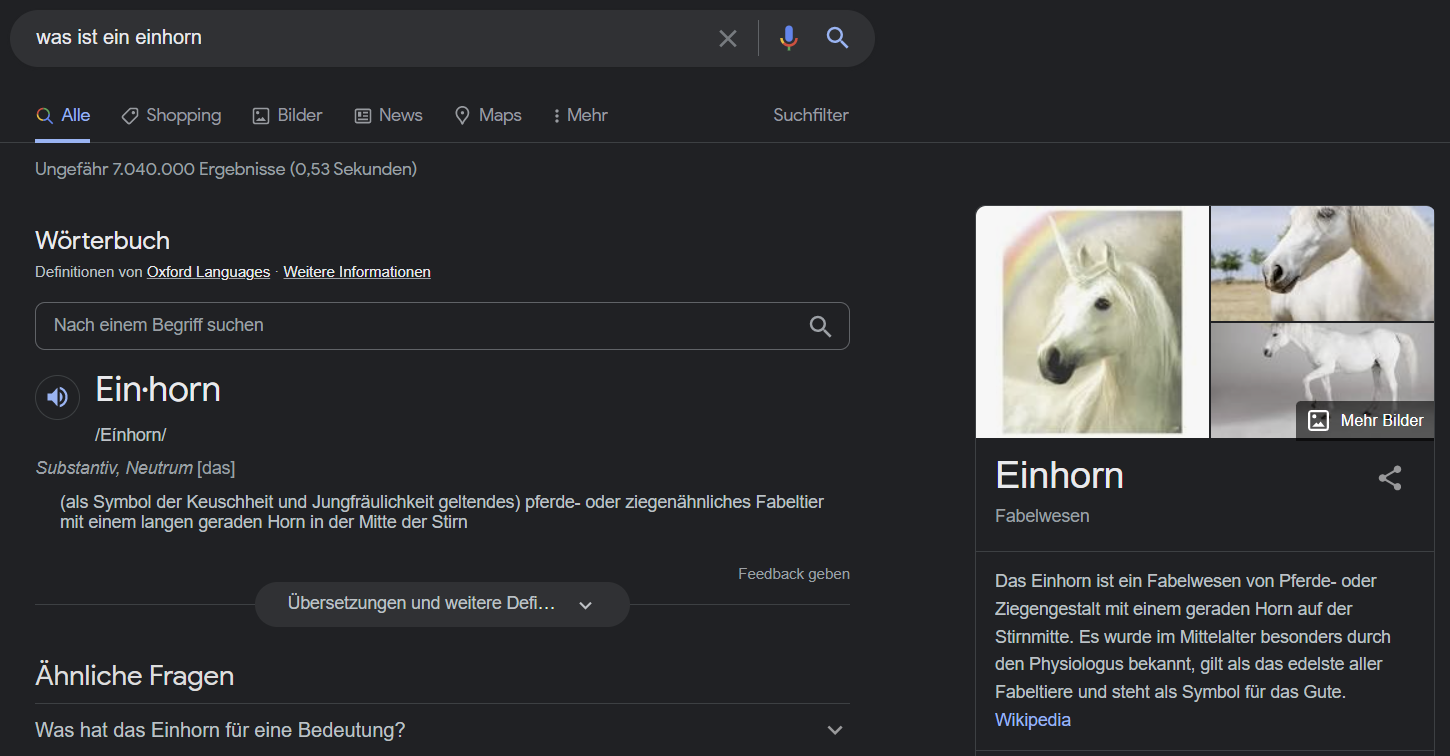
\includegraphics[width=80mm]{images/screenshot_googleQue}
    \caption{Suchergebnis Google}
    \label{fig:screenshotGoogleQue}
\end{figure}
\begin{figure}[h]
    \centering
    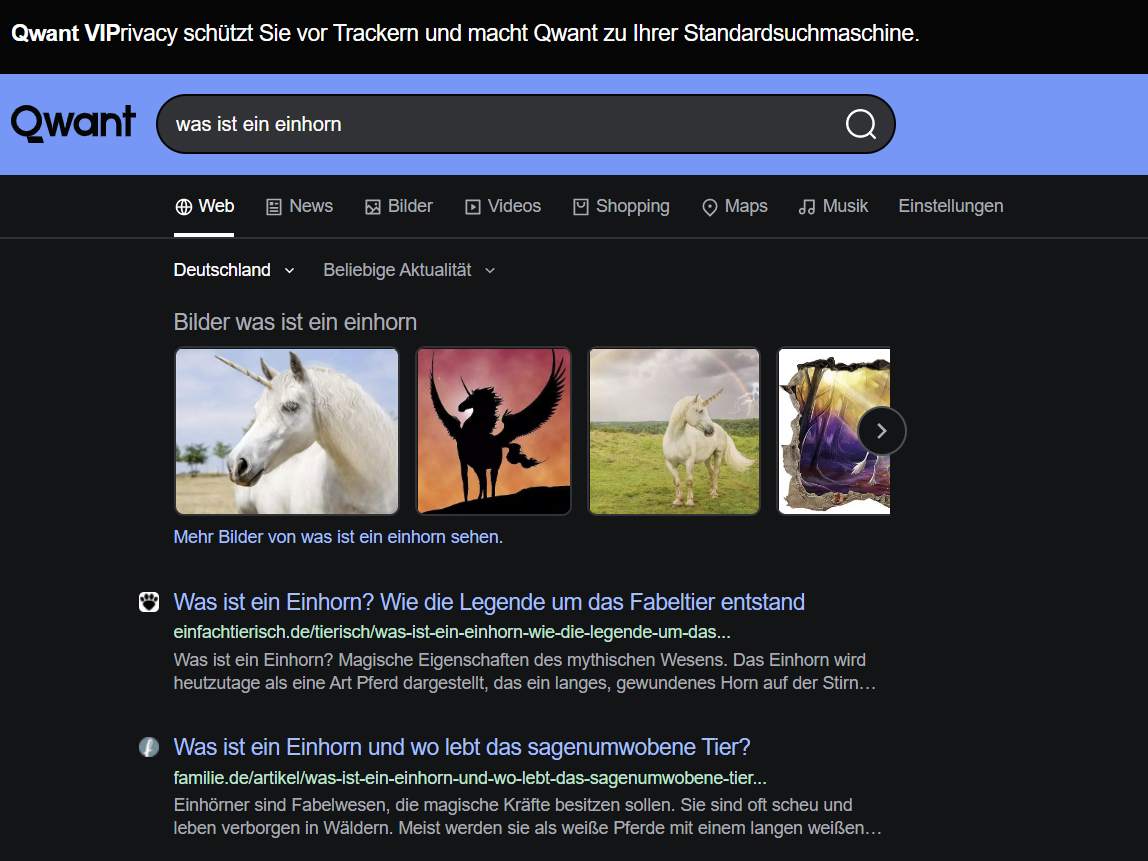
\includegraphics[width=80mm]{images/screenshot_qwantQue}
    \caption{Suchergebnis Qwant}
    \label{fig:screenshotQwantQue}
\end{figure}
Wie man in den angeführten Screenshots sieht, gibt Google direkt die Informationen aus, wo man zum Beispiel bei Qwant zuerst eine Webseite aufrufen muss.
Heute erwarten wir möglichst schnell an die Information zu kommen, worauf sich Google schon angepasst hat.

  %%%%%%%%%%%%%%%%%%%%%%% Literaturverzeichnis %%%%%%%%%%%%%%%%%%%%%%%
  \printbibliography
\addcontentsline{toc}{section}{Literatur}
\newpage


  %%%%%%%%%%%%%%%%%%%%%%%%%%%%%% Anhang %%%%%%%%%%%%%%%%%%%%%%%%%%%%%%
  \renewcommand{\thetable}{\Alph{section}.\arabic{table}}
  \renewcommand{\thefigure}{\Alph{section}.\arabic{figure}}
  \renewcommand{\thelstlisting}{\Alph{section}.\arabic{lstlisting}}
  \pagenumbering{Alph}

  \begin{appendix}
  \section{Anhang}

  \begin{figure}[h]
    \centering
    \fbox{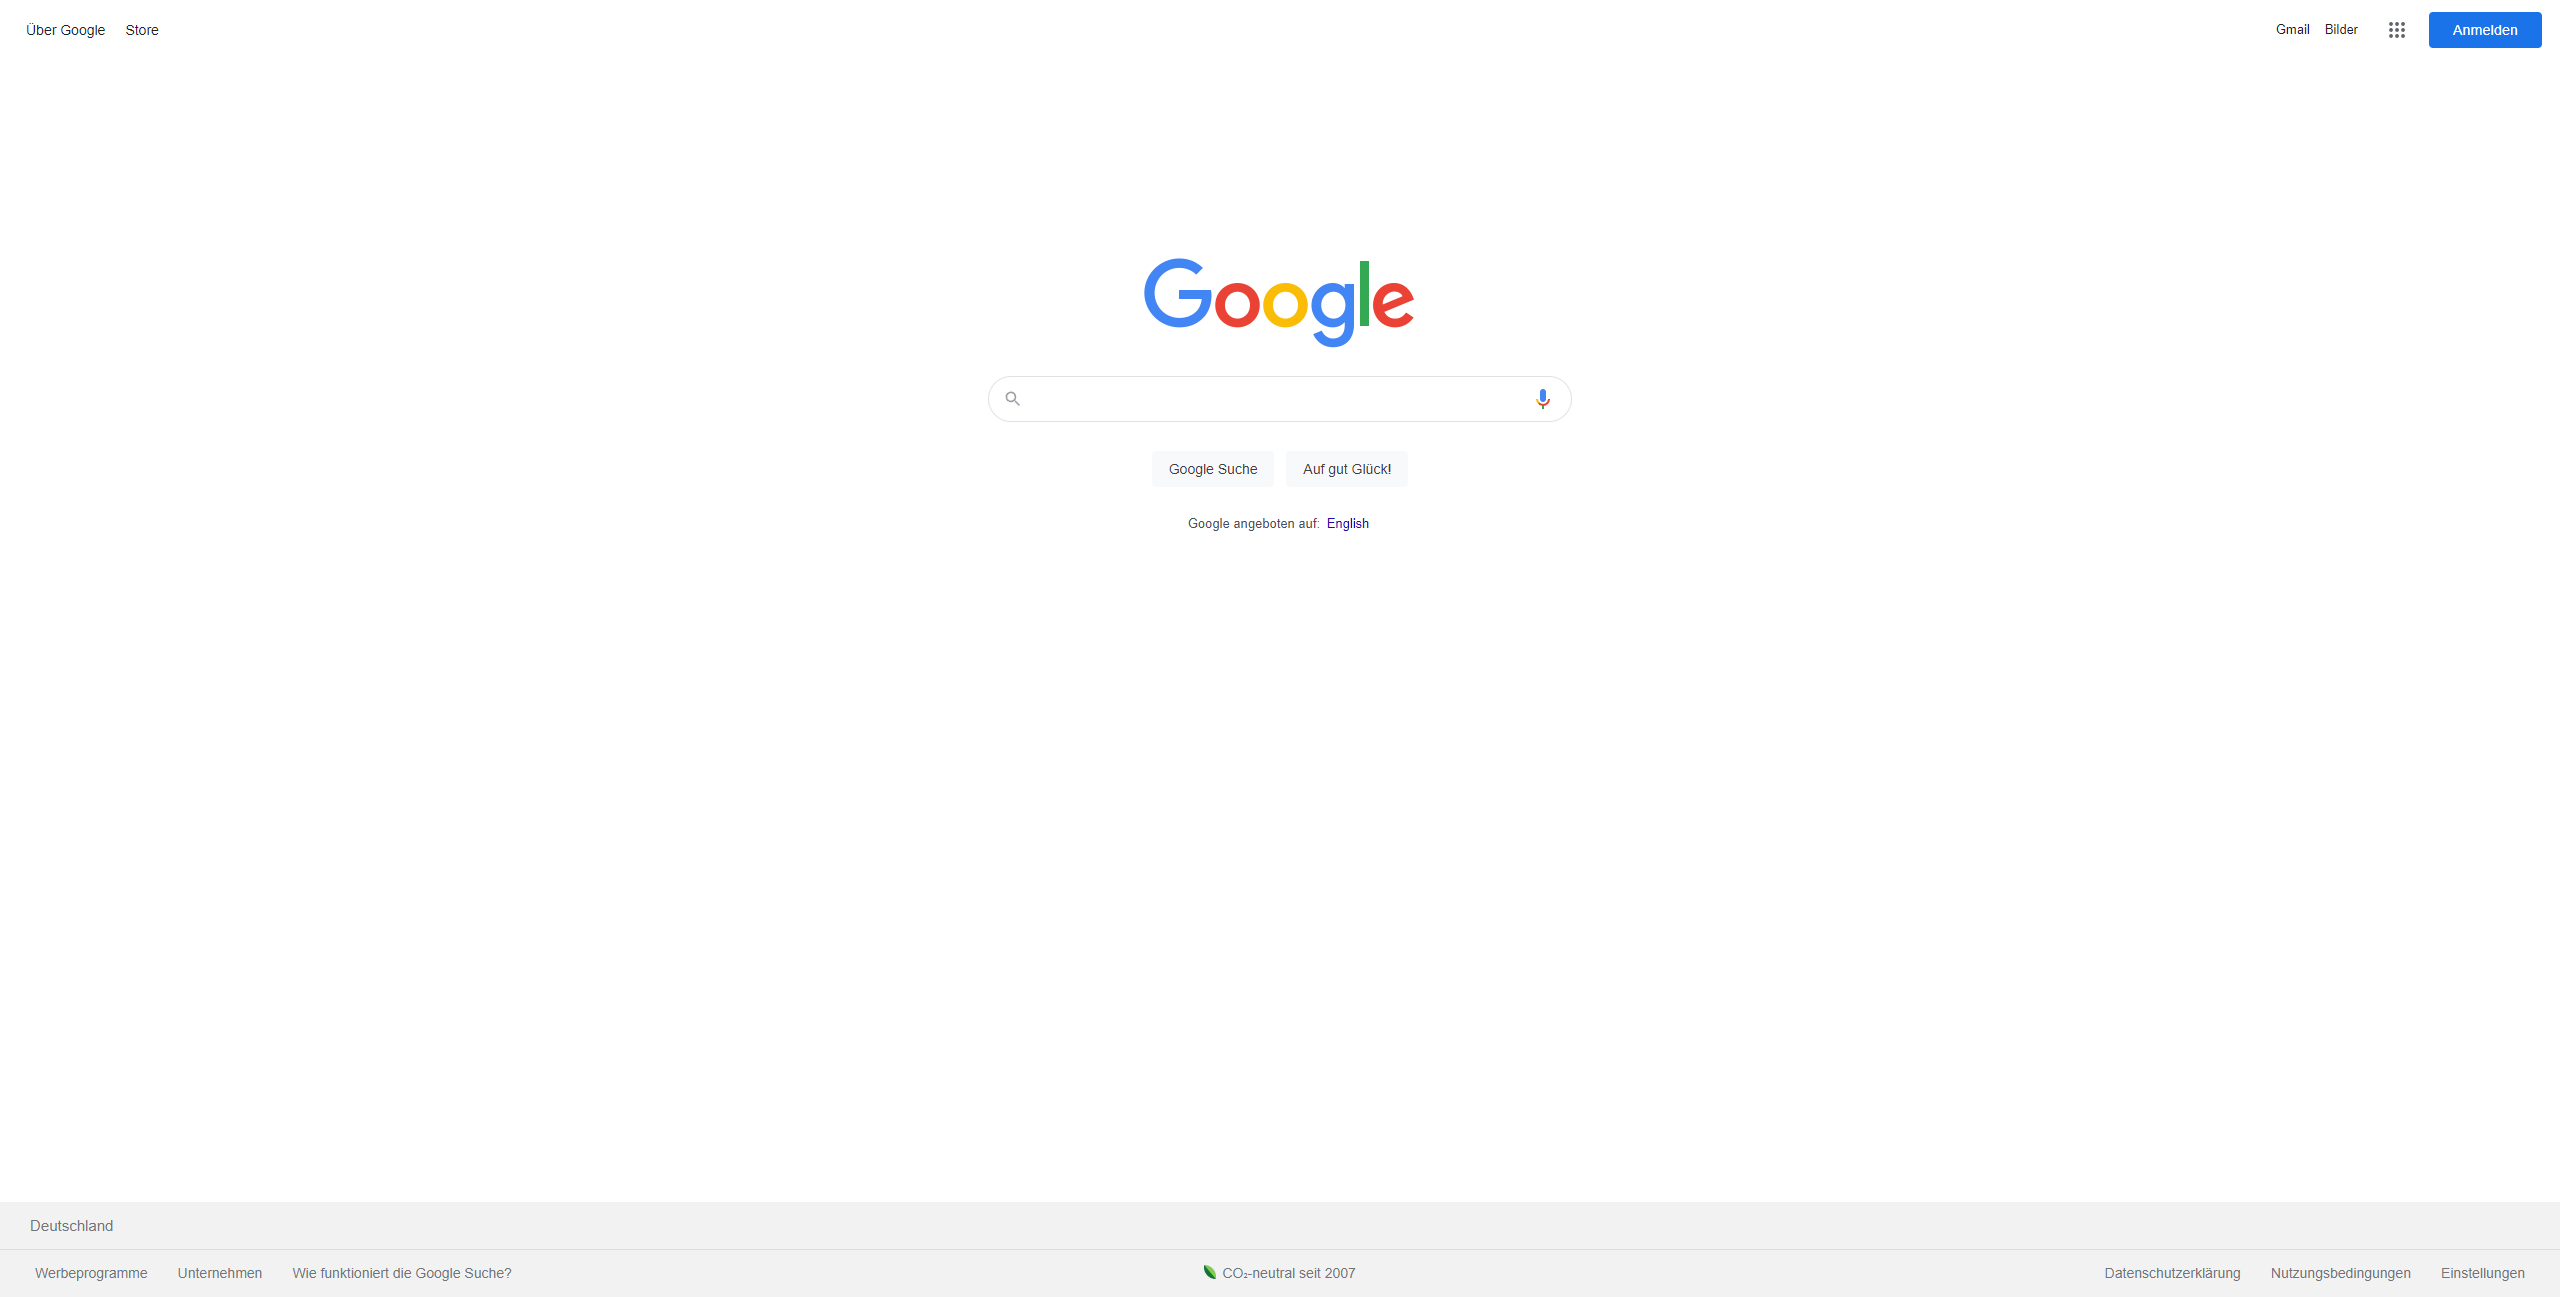
\includegraphics[height=0.3\textheight]{google_home}}\caption{Google Home}\label{fig:google_home}
  \end{figure}
  \begin{figure}[h]
    \centering
    \fbox{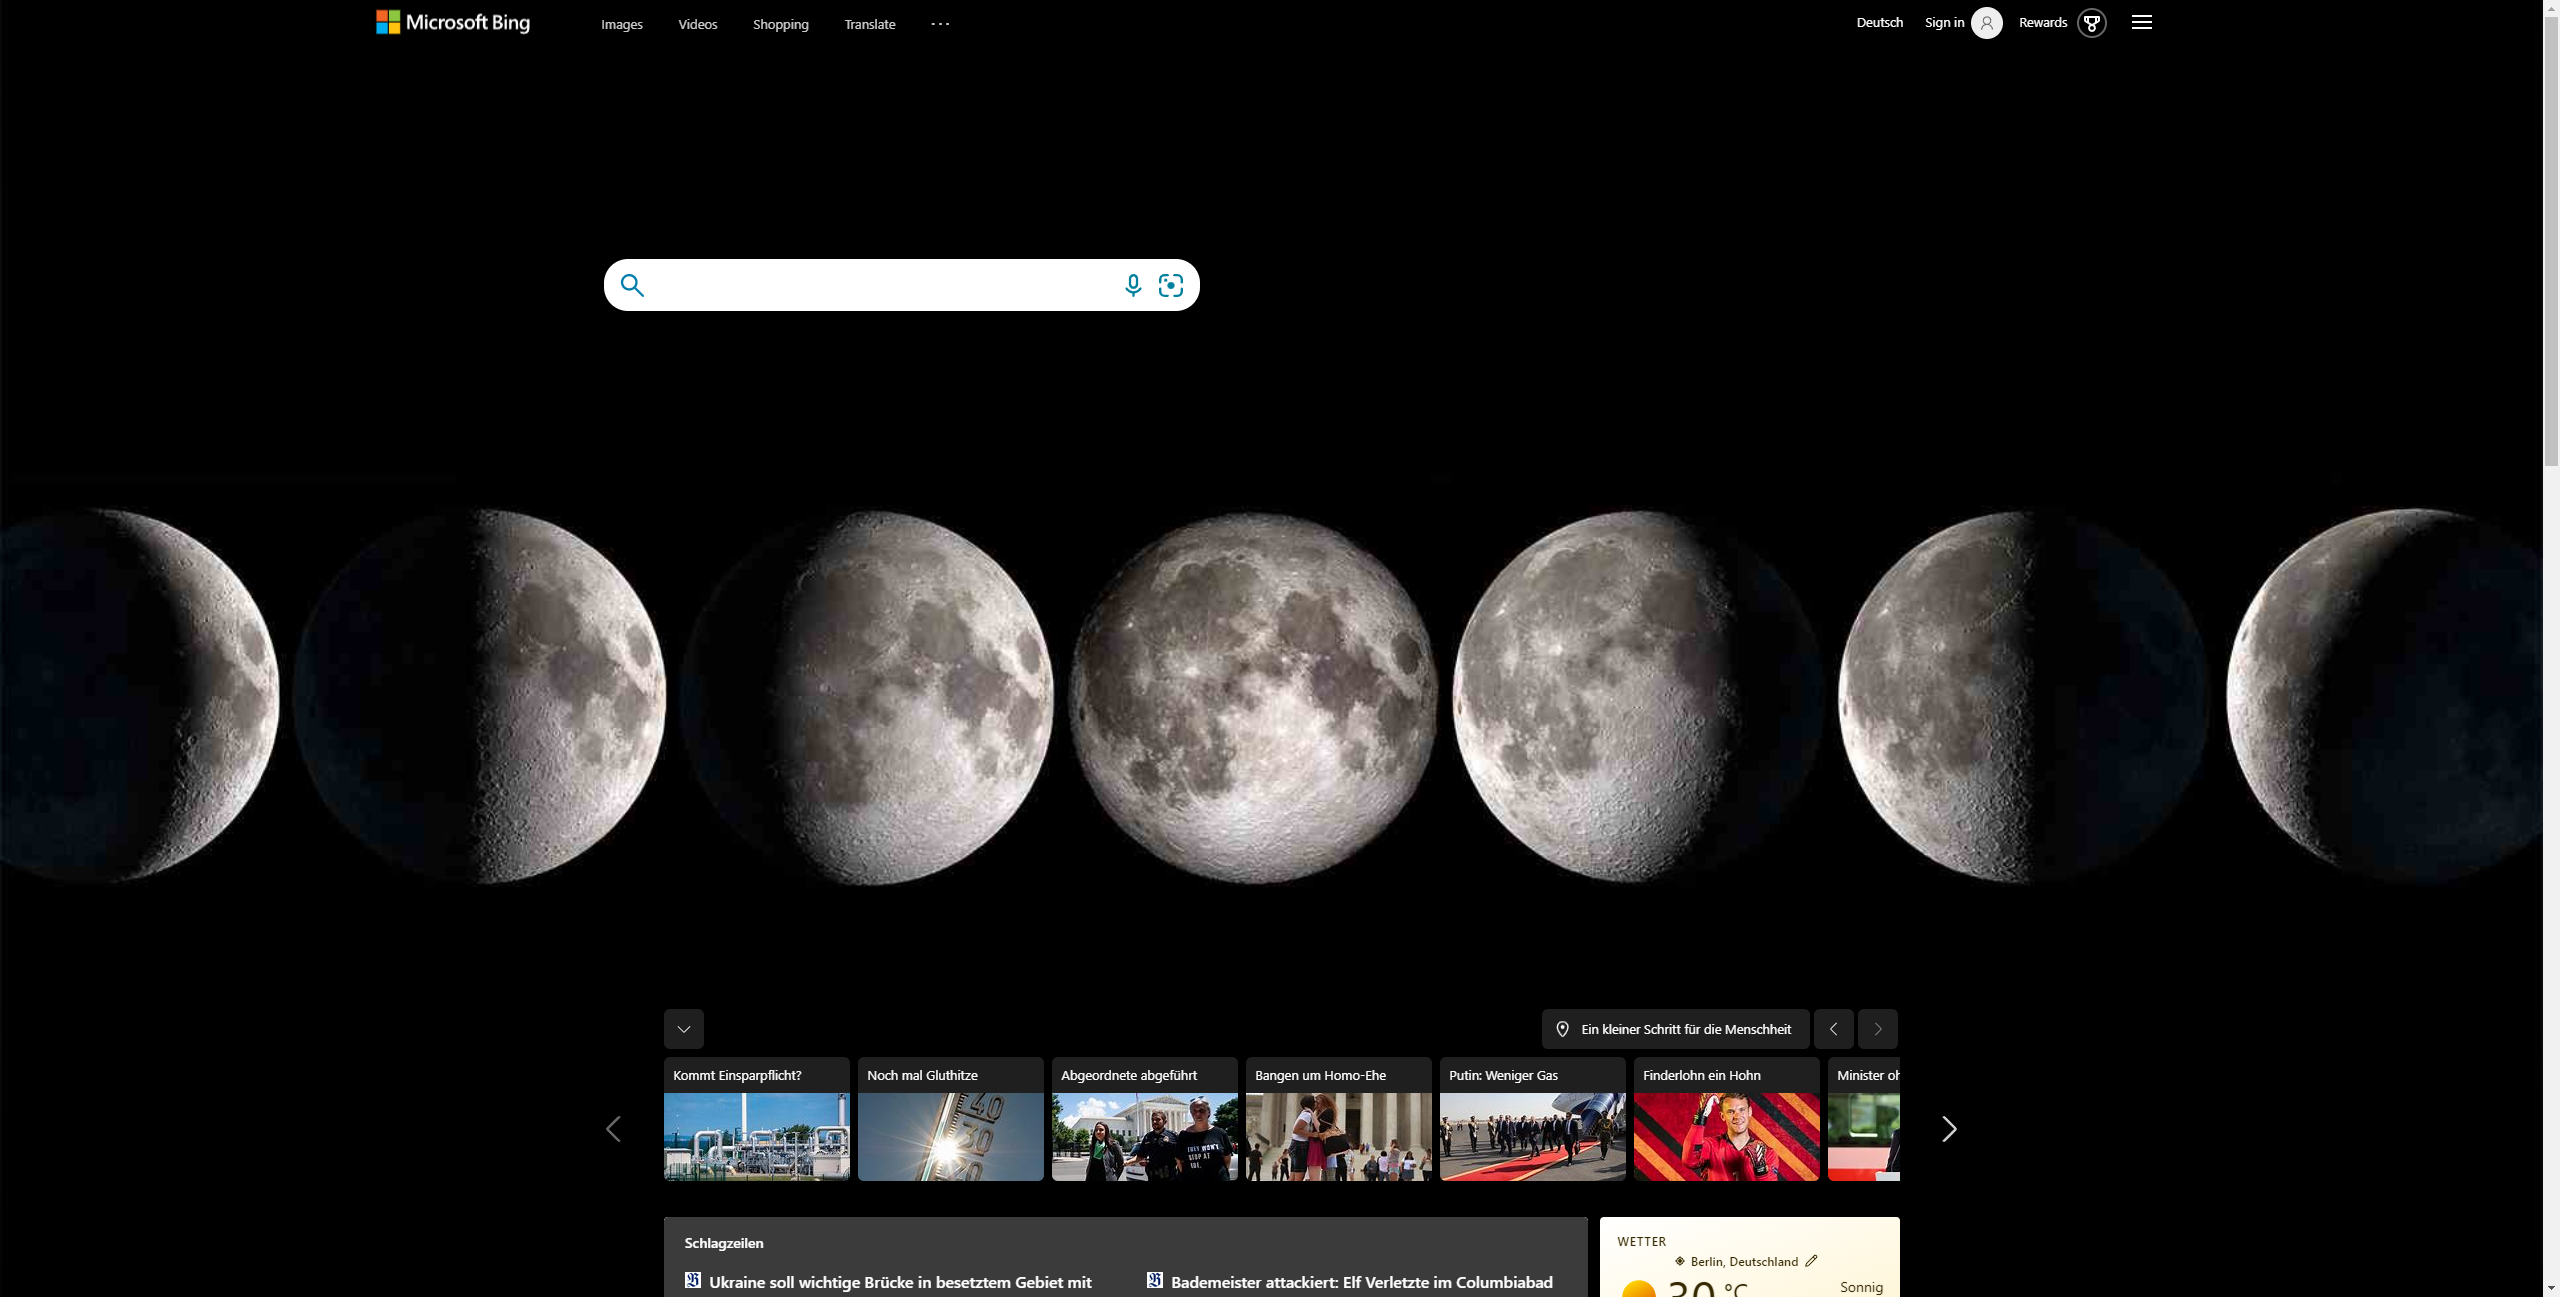
\includegraphics[height=0.3\textheight]{bing_home}}\caption{Bing Home}\label{fig:bing_home}
  \end{figure}
  \begin{figure}[h]
    \centering
    \fbox{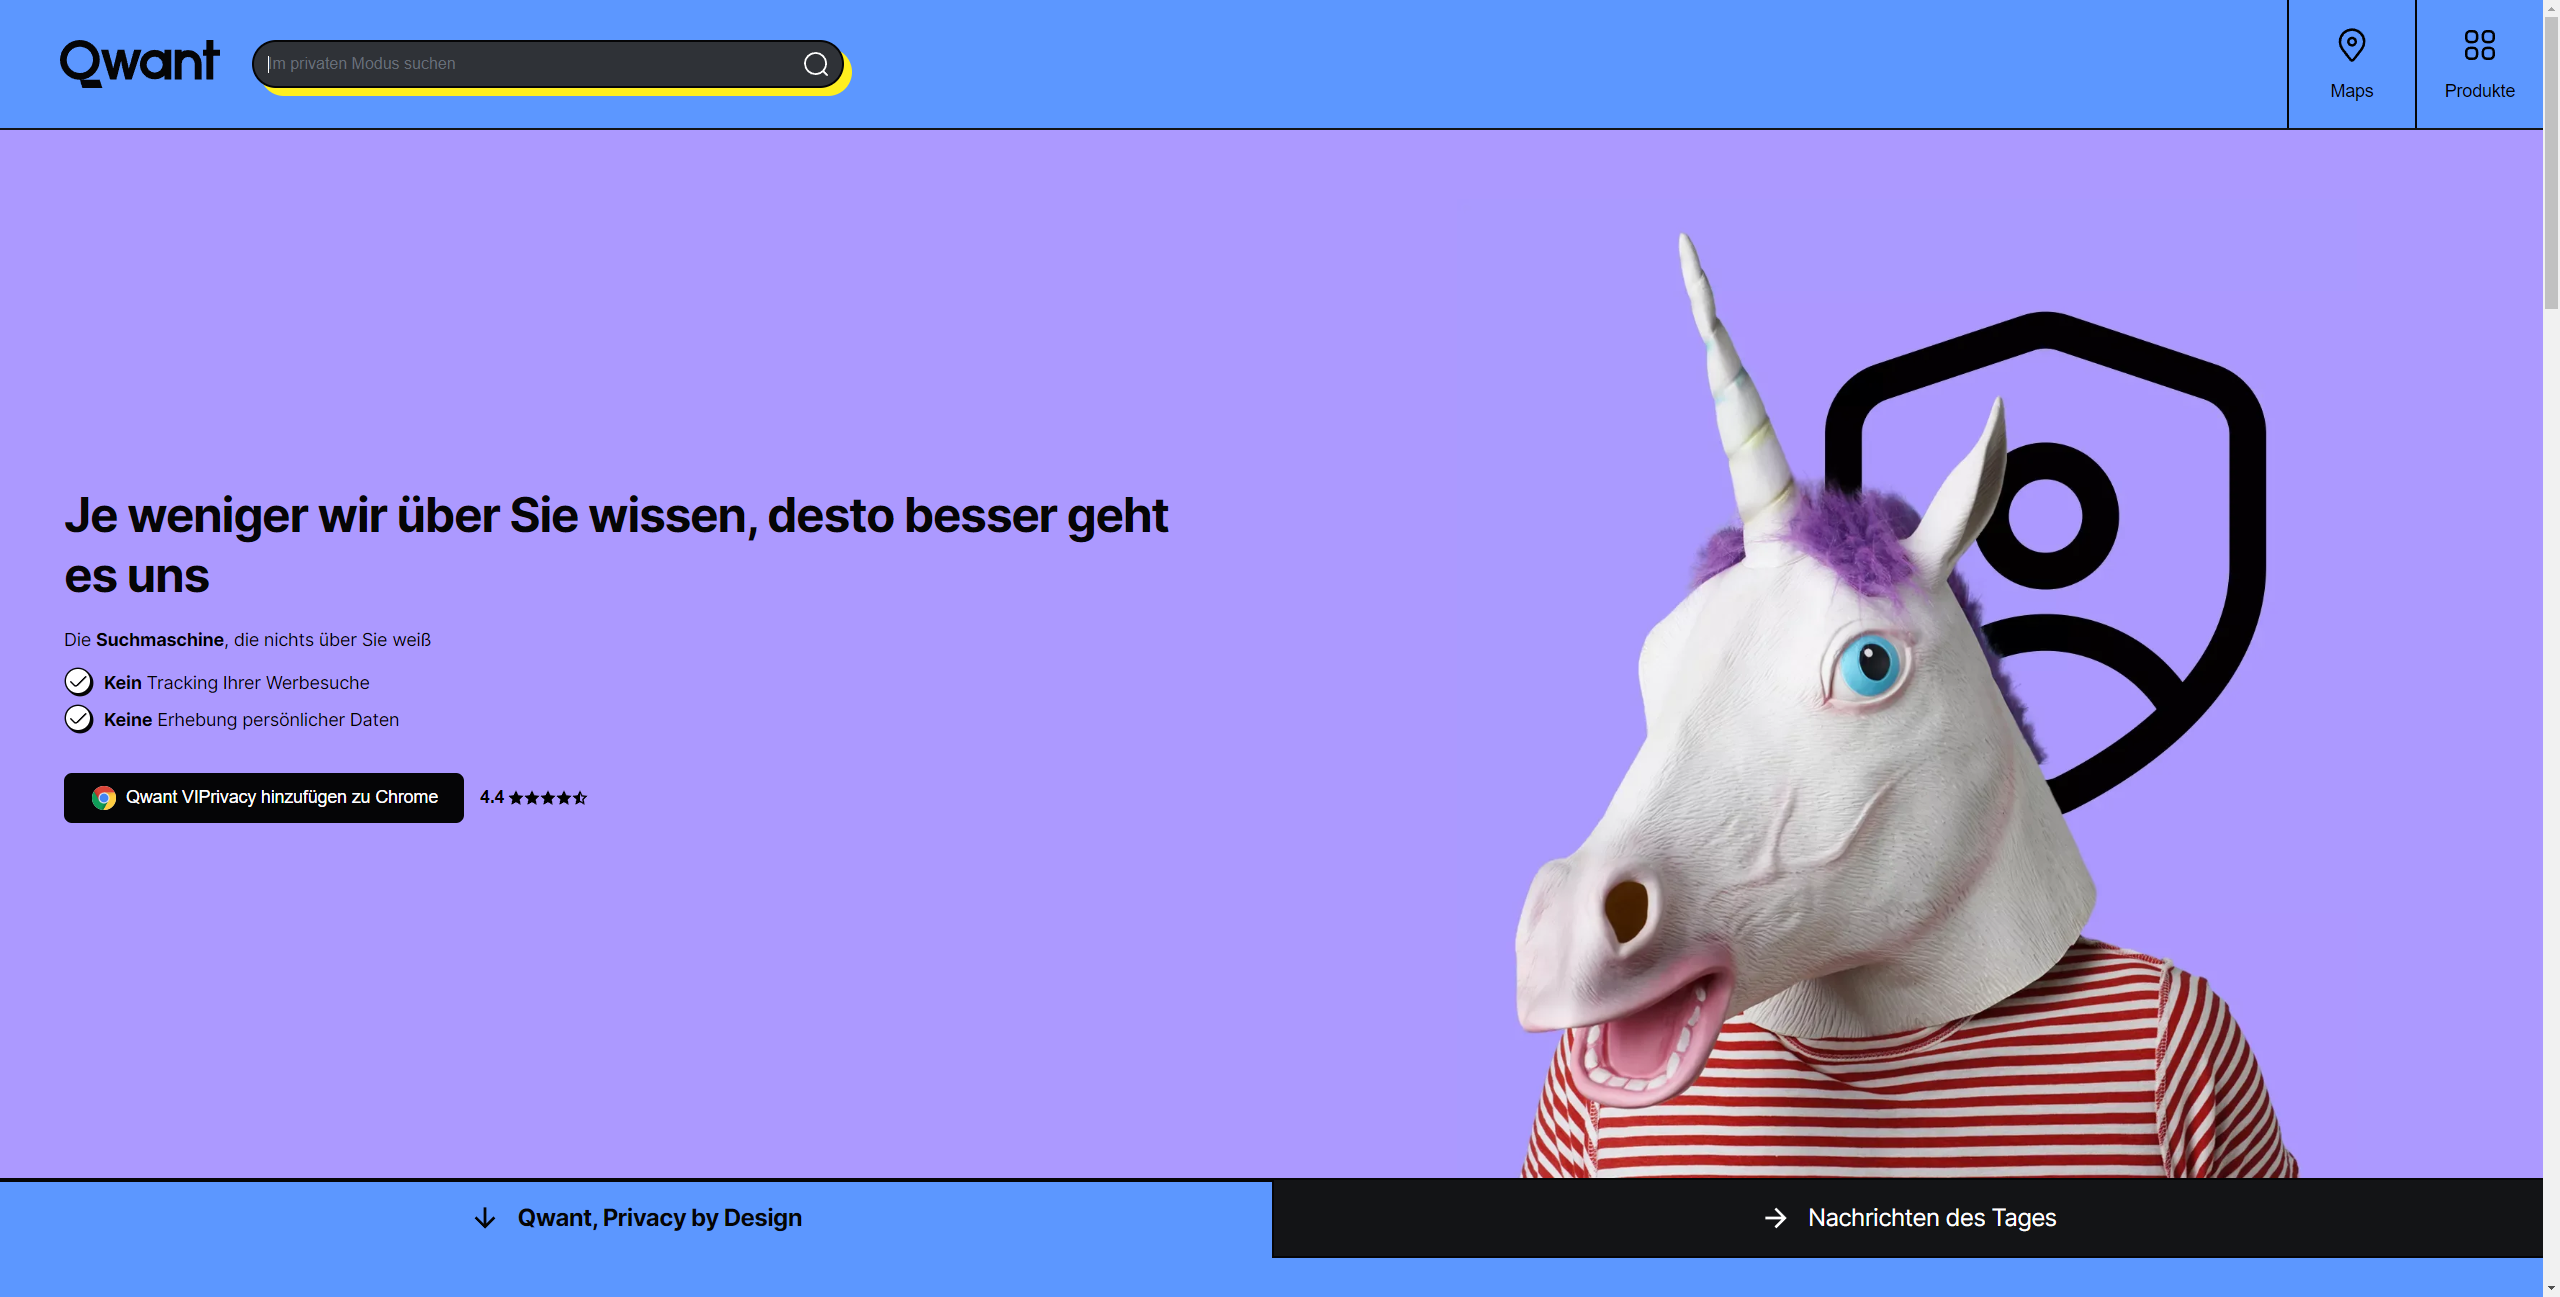
\includegraphics[height=0.3\textheight]{qwant_home}}\caption{Qwant Home}\label{fig:qwant_home}
  \end{figure}
\end{appendix}
\end{document}